% IMPORTANT NOTES TO FOLLOW OVERALL:
%A) the lab description of the respective topic (to make the report selfcontained)
%B) 1-2 pages pointing out how much they solved and which issues they encountered
%C) A “print” of an example run
%D) 1-2 pages where they relate what they did to the relevant theory in the curriculum
%E) max 1 page conclusion, concluding what was solved well (perhaps even makes you proud :-)- and what could be done differently/better and why

\section*{TCP Task Manager and Server Xml Serialization}

\subsection*{Description:}

The \textit{The Transmition Control Protocol}\textbf{TCP} is part of the core protocols of the Internet, since TPC provides with a reliable, ordered, error-checked delivery of a stream of octets between programs running on computers connected to a local network, intranet or public Internet since it resides in the transport layer.\footnote{http://java.dzone.com/articles/understanding-transport-layer}

Since web browsers uses \textbf{TCP} when they connect to the world wide web, there is the possibility to use its functionality to clients so data can be modified in the server and create task dynamically. This task manager \textbf{TCP} server offers some predefined commands that can be use to provide a service, such as:

\begin{enumerate}
\item \textbf{GET} to get items
\item \textbf{POST} to add items
\item \textbf{PUT} to update
\item \textbf{DELETE} to remove items
\end{enumerate}

\textbf{TCP} server and client follow a strict structured communication based on the following conversational protocol:

\begin{figure}[ht!]
\centering
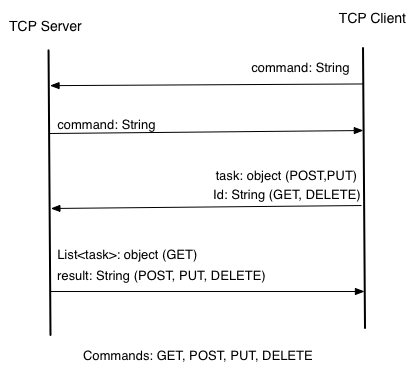
\includegraphics[width=80mm]{graphics/TCP-Server-protocol.png}
\label{overflow}
\end{figure}

%should implement elevorate more this part? hmmmm
\subsubsection*{The Task:}
Since all tasks are based of dependency of the $task-manager.xml$ file to store, read, update or delete data with subsequent task runs by Task Manager TPC Server. In this lab exercise it was require to develop the code for the following functionalities:

\begin{enumerate}
\item Develop java serialization classes for task-manager-xml using Java Architecture.
\item Develop \textit{TaskManagerTCPServer} and \textit{TaskManagerTCPClient} classes.
\end{enumerate}

%[Optional] The server described above can only handle one single client at a time in each run. In order to make the server more robust and handle multiple clients concurrently, one may follow the approach suggested in the page. 173 of the course textbook [DS], to create a new connection for every client request that will run on a separate thread. Therefore, develop a TaskManagerTCPServer that can handle multiple concurrent clients.
%
%[Optional] The functionality of TaskManagerTCPServer can be extended to offer more commands (e.g. OPTIONS, HEAD) similar to the HTTP protocol. In case of OPTIONS command, one may describe the list of commands offered by the server, where as for HEAD, one may only provide the number of tasks available for a given attendant instead of sending all the available tasks to the client.

\subsection*{Solutions:}

\begin{lstlisting}[language=java]
	public class TcpClient {
	//extends how it is created
	//which method it takes. parameter
	//security ,improvements
	//how handle multiple requests
\end{lstlisting}

\subsection*{Conclutions:}